% \documentclass[../Main.tex]{subfiles}
% \externaldocument{0.0.overview}



% \begin{document}
\chapter{用于快速采样的基于蒸馏的方法}\label{ch:distillation}

本章介绍基于训练的方法，通过训练新的生成器使其仅需一步或几步即可产生样本，从而加速扩散模型的采样。其核心思想被称为\emph{蒸馏}（distillation），即让一个快速的学生模型（student model）向一个缓慢、预训练好的扩散模型（教师模型，teacher）采样器学习。虽然教师模型可能需要数百步，学生模型却能在仅需几步的情况下达到可比的质量\footnote{此处蒸馏指的是减少采样步数，而非缩小模型规模。}。与改进数值积分格式的求解器加速不同，蒸馏直接训练生成器走高效的捷径。我们重点介绍两种主要范式：\emph{分布级蒸馏}（distribution level distillation），它跳过对完整轨迹的模拟，转而使学生模型的输出分布与教师模型的分布对齐；以及\emph{流映射级蒸馏}（flow map level distillation），它训练学生模型以更快、更紧凑的方式复现教师模型的采样路径。

% This chapter introduces training-based methods for obtaining a one- or few-step denoiser (generator) for fast sampling by assuming an access to some well-trained pre-trained DM $\rvs_{\bm{\phi}^\times}(\rvx_s, s) \approx \nabla_{\rvx_s} \log p_s(\rvx_s)$. With the pre-trained DM, it can provides a proxy to $p_{\mathrm{data}}$ via sampling trajectory (i.e., SDE/ODE solving) as highlighted in \Cref{subsec:sde-sample}. the  The high-level idea of common approaches is either to distill the trajectory, or the learned distributions of a pre-trained diffusion model (teacher) into a fewer-steps generator from noise to a clean estimate.




% , which is supposed to be a proxy to $p_{\mathrm{data}}$ while sampling from its requires SDE/ODE solving as highlighted in \Cref{subsec:sde-sample}. Many approaches were proposed to extract either its sampling trajectory (we call it \emph{Trajectory Distillation}) into a few step generators or extract distribution modeled by the pre-trained DM (we refer to \emph{Distributional Distillation})
\clearpage
\newpage


\section{引言}\label{sec:distillation-prologue}
扩散模型的一个核心瓶颈是其缓慢的采样速度。

如 Tweedie 公式（\Cref{subsec:four-equiv-para}）所示，扩散模型可以解释为一个“$\rvx$-预测”模型 $\rvx_{\bm{\phi}^\times}(\rvx_t, t)$，它被训练为在噪声水平 $t$ 下从带噪输入 $\rvx_t$ 恢复期望的干净数据：
\[
    \rvx_{\bm{\phi}^\times}(\rvx_t, t) \approx \mathbb{E}[\rvx_0 |\rvx_t],
\]
其中期望是关于 $p(\rvx_0 |\rvx_t)$ 取的，表示与 $\rvx_t$ 对应的所有可能干净数据。
一个自然的想法是用 $\rvx_{\bm{\phi}^\times}(\rvx_t, t)$ 进行一步生成。但由于该去噪器对许多可能结果进行了平均，预测会变得过度平滑，仅用少量去噪步骤进行生成会导致模糊、低质量的样本。

另一方面，如 \Cref{subsec:sde-sample} 所讨论的，扩散采样沿 ODE 或 SDE 轨迹经历一长串迭代步骤。这产生了高保真度的样本，但所需的大量步数使得该过程本质上是缓慢的。降低 NFE（即采样步数乘以模型调用次数）可以加快生成，但不可避免地会降低保真度。
每个求解器步长都引入 $\mathcal{O}(h^{n})$ 阶的积分误差，
其中 $n$ 是求解器阶数，$h=\max_i |t_i - t_{i-1}|$ 是步长。
步数越少意味着时间增量 $h$ 越大，这又反过来增加了累积的采样误差，导致轨迹精度下降。
这在扩散采样的质量与效率之间造成了根本性的权衡。

为克服这一瓶颈，一条重要的研究路线是\emph{蒸馏}，它假设可以访问一个训练良好的扩散模型（\emph{教师模型}），并训练一个生成器（\emph{学生模型}）通过单次前向或几步计算来复现其行为。
这把教师模型的许多采样步骤压缩成一个快速过程，在保持高样本保真度的同时有效地绕过了缓慢的迭代求解器。




下面，我们介绍关于蒸馏的两种视角：\emph{分布级蒸馏}和\emph{流映射级蒸馏}\footnote{从时间顺序上看，以 \emph{Knowledge Distillation}（KD）~\citep{luhman2021knowledge} 和 \emph{Progressive Distillation}（PD）~\citep{ho2020denoising} 为代表的流映射级蒸馏更早于 2021 年提出，早于 2023 年前后兴起的分布级蒸馏方法家族。不过，为了叙述更顺畅并与下一章衔接，我们先介绍分布级蒸馏。}。




\subsection{分布级蒸馏}
基于分布的蒸馏的目标是训练一个单步生成器 $\rmG_{\bm{\theta}}(\rvz)$，它将噪声 $\rvz \sim p_{\mathrm{prior}}$ 映射到样本 $\hat\rvx = \rmG_{\bm{\theta}}(\rvz)$，从而诱导一个分布 $p_{\bm{\theta}}(\hat\rvx)$，用以逼近目标数据分布 $p_{\mathrm{data}}(\rvx)$。这通常通过最小化某个统计散度来实现
\[
\min_{\bm{\theta}}  \mathcal{D}\!\left(p_{\bm{\theta}}(\hat\rvx),  p_{\mathrm{data}}(\hat\rvx)\right),
\]
其中 $\mathcal{D}$ 表示某个合适的散度度量，例如 KL。

在实践中，基于分布的方法将生成器的分布与预训练扩散模型所产生的经验分布 $p_{\bm{\phi}^\times}(\rvx)$ 对齐：
\[
\min_{\bm{\theta}}  \mathcal{D}\!\left(p_{\bm{\theta}}(\hat\rvx),  p_{\bm{\phi}^\times}(\hat\rvx)\right),
\]
其中 $p_{\bm{\phi}^\times}$ 充当 $p_{\mathrm{data}}$ 的代理。这些方法并不显式地计算该散度，而是逼近其梯度，而该梯度可以直接从预训练教师模型计算得到。
这使得学生模型能够将其分布与教师模型对齐，而无需完整的散度求值。

这一表述通过分布对齐将扩散模型的多步生成过程蒸馏为单步模型。我们在 \Cref{sec:VSD} 中详细阐述该方法。




\subsection{流映射级蒸馏} 我们考虑 PF-ODE，它可以用任意预测模型表示（见 \Cref{eq:predictions-equivalence}）：
\begin{align}\label{eq:pf-ode-ct}
    \frac{\diff \rvx(\tau)}{\diff \tau} 
    = f(\tau) \rvx(\tau) - \tfrac{1}{2}g^2(\tau) \nabla_\rvx \log p_\tau(\rvx(\tau)) 
    =: \rvv^*(\rvx(\tau), \tau).
\end{align}

其解映射记为 $\bPsi_{s\to t}(\rvx_s)$，表示从时间 $s$ 的 $\rvx_s$ 出发反向演化到时间 $t \leq s$；即
\begin{align}\label{eq:int_target_gt}
\begin{aligned}
    \bPsi_{s\to t}(\rvx_s) 
    &\coloneqq \rvx_s + \int_s^t \rvv^*(\rvx(\tau), \tau) \diff \tau,
\end{aligned}
\end{align}
其中积分求解的是 PF-ODE。直观地说，$\bPsi_{s\to t}$ 将时间 $s$ 的噪声 $\rvx_s$ 输运到时间 $t$ 处噪声更少的状态（最终在 $t=0$ 时成为数据）。


从扩散模型采样对应于对 $\rvx_T \sim p_{\mathrm{prior}}$ 求值 $\bPsi_{T\to 0}(\rvx_T)$。通常，该积分由利用速度场 $\rvv$ 的迭代数值求解器逼近（见 \Cref{ch:solvers}），但需要许多步（例如 DPM-Solver 中至少 $10$ 步），使得采样比 GAN 等经典单步生成模型更慢。这引出一个自然的问题：
\begin{question}
    我们能否直接学习解映射 $\bPsi_{s\to t}(\rvx_s)$？
\end{question}
特别地，学习映射 $\bPsi_{T\to 0}(\rvx_T)$（其中 $\rvx_T \sim p_{\mathrm{prior}}$）即可实现单步生成。


\paragraph{轨迹蒸馏。}

轨迹蒸馏旨在训练一个神经生成器，在实例层面逼近解映射。由于 PF-ODE 积分很少有闭式形式，训练时必须对其进行数值逼近。为形式化，我们引入通用的求解器记号
\begin{align}\label{eq:solver}
    \mathtt{Solver}_{s\to t}(\rvx_s;\,\bm{\phi}^\times)
    \quad \text{or simply} \quad
    \mathtt{Solver}_{s\to t}(\rvx_s),
\end{align}
表示从 $s$ 到 $t$、以 $\rvx_s$ 为起点对经验 PF-ODE 进行数值积分，
使用教师参数 $\bm{\phi}^\times$（在上下文清楚时省略）。



\paragraph{一种早期方法：直接知识蒸馏。}
为了实现少步乃至单步生成，一种直接的方法是训练一个生成器 $\rmG_\btheta(\rvx_T, T,0)$，去模仿沿完整轨迹求值的数值求解器输出：
\[
\rmG_\btheta(\rvx_T, T,0)\approx \mathtt{Solver}_{T\to 0}(\rvx_T), 
\qquad \rvx_T \sim p_{\mathrm{prior}}.
\]
这一思想是早期轨迹蒸馏方法之一——\emph{知识蒸馏}（Knowledge Distillation）~\citep{luhman2021knowledge} 的基础，它使用回归损失
\[
\mathcal{L}_{\mathrm{KD}}(\btheta)
:= 
\E_{\rvx_T \sim p_{\mathrm{prior}}}
\left\|
\rmG_\btheta(\rvx_T, T,0)
-
\mathtt{Solver}_{T\to 0}(\rvx_T)
\right\|_2^2.
\]
虽然该方法能提供来自预训练教师模型的直接监督，
但它无法利用原始训练数据中可获得的强监督。
此外，若在训练循环中调用 ODE 积分，计算开销会非常昂贵，因为每次参数更新都需要求解 ODE 来构造目标。
最后，由于生成器只学到从 $T$ 到 $0$ 的全局映射，它可能会失去从中间状态操控生成过程的可控性。因此，\Cref{ch:guidance} 中介绍的大多数可控生成技术无法直接应用。




\paragraph{渐进式蒸馏的前言。}
\emph{渐进式蒸馏}（Progressive Distillation，PD）~\citep{salimans2021progressive} 使用来自 $\mathtt{Teacher}$ 片段的\emph{局部}监督来训练一个时间条件化的 $ \mathtt{Student} $。
设 $t_0=T>t_1>\cdots>t_N=0$ 为固定的时间网格。
$ \mathtt{Teacher} $ 为 $k=0,\ldots,N-1$ 提供时间步进映射 $\mathtt{Teacher}_{t_k\to t_{k+1}}$。


PD 并非只监督单跳 $T\to 0$，而是训练 $ \mathtt{Student}  $ 的两步跨越映射来匹配两个连续的 $ \mathtt{Teacher}$ 步：
\[
\mathtt{Student}_{t_k\to t_{k+2}}
\;\approx\;
\mathtt{Teacher}_{t_{k+1}\to t_{k+2}}
\circ
\mathtt{Teacher}_{t_{k}\to t_{k+1}},
\]
其中 $k = 0, 2, 4, \dots$。
匹配使用简单的回归损失（如均方误差）。


在局部配对片段上训练之后，$ \mathtt{Student} $ 不再沿原始网格的每个时间区间前进。
相反，它在每隔一个时间点上前进，
\[
t_0 \to t_2 \to t_4 \to \cdots \to t_N,
\]
这意味着每个 $ \mathtt{Student} $ 步实际上覆盖了两个连续的 $ \mathtt{Teacher}$ 步。
因此，$ \mathtt{Student} $ 仅用 $N/2$ 次转移即可完成相同的总时间跨度 $[0,T]$。

在此阶段之后，训练好的 $ \mathtt{Student} $ 取代 $ \mathtt{Teacher}$，作为新的参考模型。
然后整个流程在更稀疏的网格上重复，时间步长加倍
$(N \to N/2 \to N/4 \to \cdots)$，
逐步将轨迹蒸馏为越来越少的步数，直到达到所需的推理步数。
这种迭代式减半在保持全局时间跨度的同时，不断压缩生成过程的时间分辨率。






\paragraph{流映射学习的统一视角。}
包括 KD 和 PD 在内的多种方法都可以纳入统一的损失框架：
\begin{align}\label{eq:general-cm-loss}
  \mathcal{L}_{\mathrm{oracle}}(\btheta)
  := \E_{s,t} \E_{\rvx_s \sim p_s} 
  \left[  w(s,t)  d \big(\rmG_\btheta(\rvx_s, s,t),  \bPsi_{s\to t}(\rvx_s)\big)\right],
\end{align}
其中 $\bPsi_{s\to t}$ 是 oracle 流映射，$w(s,t) \geq 0$ 指定不同时间对 $(s,t)$ 的加权方式，
$d(\cdot,\cdot)$ 是差异度量，例如
$d(\rvx,\rvy)=\|\rvx-\rvy\|_2^2$ 或 $d(\rvx,\rvy)=\|\rvx-\rvy\|_1$，而 $p_s$ 表示时间 $s$ 处前向加噪的边缘分布。由于 $\bPsi_{s\to t}$ 没有闭式表达，
必须依赖近似，通常通过预训练扩散模型（教师模型）或其他可处理的代理。

KD 表现为
\Cref{eq:general-cm-loss} 的一个简单实例。选取退化的加权
$w(s,t)=\delta(s{-}T)\,\delta(t{-}0)$ 并使用先验分布
$p_T=p_{\mathrm{prior}}$\footnote{该假设在 $T$ 足够大或采用合适的噪声调度 $(\alpha_t,\sigma_t)$ 时成立。}，oracle 损失 $\mathcal{L}_{\mathrm{oracle}}(\btheta)$ 简化为：
\[
\E_{\rvx_T\sim p_T}
\big\|\rmG_\btheta(\rvx_T,T,0)-\bPsi_{T\to 0}(\rvx_T)\big\|_2^2
\approx \mathcal{L}_{\mathrm{KD}}(\btheta),
\quad
\]
其中 $\mathtt{Solver}_{T\to 0}\approx\bPsi_{T\to 0}$。\Cref{app-sec:flow-map} 给出了该表述的另一种视角。


PD 也符合这一模板，但它并非只用单个极端时间对 $(T,0)$ 进行监督，而是使用许多\emph{邻近}的时间对，并施加一个简单的\emph{局部一致性}规则：
一次短步接着另一次短步应当匹配直接的两步移动。我们在 \Cref{eq:pd-local} 中再回到这一点。

在实践中，主要挑战在于 oracle 流映射 $\bPsi_{s\to t}$ 通常没有闭式表达，使得直接监督不可行。已有多种方法被开发出来以高效地逼近这一
目标，但它们的成功往往取决于教师模型
的质量。我们将在 \Cref{ch:fast-scratch} 中再次回到 \Cref{eq:general-cm-loss}，提出一个用于从头训练方法的原理性框架，将教师模型从学习循环中去除。









\clearpage
\newpage



\section{\texorpdfstring{基于分布的蒸馏}{Distribution-Based Distillation}}\label{sec:VSD}


多项工作在不同名称下并行开展了基于分布的蒸馏研究，
包括 Distributional Matching Distillation（DMD）~\citep{yin2024one,yin2024improved}、
Variational Score Distillation（VSD）~\citep{pooledreamfusion,wang2023prolificdreamer,luo2023diff,lu2024simplifying}
和 Score Identity Distillation（SiD）~\citep{zhou2024score}。
尽管技术细节有所不同，它们共享同一原理：
训练一个生成器，使其前向加噪后的边缘分布与教师模型相匹配。
我们以 VSD 作为代表性表述重点介绍，因为其他方法遵循类似的原理。


\subsection{作为代表性方法的 VSD 表述}
\paragraph{前向过程。}
设 $\{p_t\}_{t \in [0,T]}$ 表示由下式诱导的前向扩散过程的边缘密度
\[
\rvx_t = \alpha_t \rvx_0 + \sigma_t \bm{\epsilon}, \quad \bm{\epsilon} \sim \mathcal{N}(\bm{0}, \rmI),
\]
其初始分布为 $p_0 = p_{\mathrm{data}}$。
相反地，设 $p_0^{\bm{\theta}}$ 为确定性单步生成器 $\rmG_{\bm{\theta}}(\rvz)$ 从隐变量 $\rvz \sim p_{\mathrm{prior}}(\rvz)$ 生成的合成样本所构成的分布。定义 $\{p_t^{\bm{\theta}}\}_{t \in [0,T]}$ 为对 $p_0^{\bm{\theta}}$ 施加相同前向扩散过程所得到的边缘密度，即
\begin{align}\label{eq:vsd-forward}
    \rvx_t^{\bm{\theta}} := \alpha_t \rmG_{\bm{\theta}}(\rvz) + \sigma_t \bm{\epsilon}, 
\end{align}
其中 $\rvz \sim p_{\mathrm{prior}}$，$ \bm{\epsilon} \sim \mathcal{N}(\bm{0}, \rmI)$。因此，$p_t$ 和 $p_t^{\bm{\theta}}$ 共享同一高斯扩散核
$p_t(\rvx_t| \rvx_0)$，但起始分布不同
（分别为 $p_{\mathrm{data}}$ 与单步合成样本的 $p_0^{\bm{\theta}}$）。

\paragraph{训练目标与梯度。}
文献中通常采用 KL 散度来匹配分布 $p_t$ 与 $p_t^{\bm{\theta}}$，一般通过最小化
\begin{align*}
    \mathcal{L}_{\text{VSD}}(\bm{\theta}) &:=\mathbb{E}_t \left[ \omega(t)  \mathcal{D}_{\text{KL}}(p_t^{\bm{\theta}} \, \| \, p_t) \right]
\\&= \mathbb{E}_{t, \rvz, \bm{\epsilon}} \left[ \omega(t) \left( \log p_t^{\bm{\theta}}(\rvx_t^{\bm{\theta}}) - \log p_t(\rvx_t^{\bm{\theta}}) \right) \right],
\end{align*}
其中 $\omega(t)$ 是时间相关的加权函数。我们将在 \Cref{subsec:vsd-discussion} 讨论 KL 散度为何在分布级蒸馏中
扮演特殊角色。



如 \citep{wang2023prolificdreamer} 所示，最优解在 $ p_0^{\bm{\theta}^*} = p_{\mathrm{data}} $ 时取得，这表明生成器的分布与数据分布匹配，因此该训练目标是学习数据分布的有效损失。

然而，基于密度的目标表述缺乏高效的训练机制。幸运的是，对 $\bm{\theta}$ 求梯度，我们得到 \Cref{eq:vsd-grad} 中的表达式，下面以命题形式总结。为记号简洁，我们将 \Cref{eq:vsd-forward} 中定义的 $\rvx_t^{\bm{\theta}}$ 记为 $\hat\rvx_t$。




\proppp{$\mathcal{L}_{\text{VSD}}$ 的 $\bm{\theta}$-梯度}{vsd-grad}{
我们有
\begin{align}\label{eq:vsd-grad}
\begin{aligned}
        &\nabla_{\bm{\theta}}\mathcal{L}_{\text{VSD}}(\bm{\theta}) \\= &\mathbb{E}_{t, \rvz, \bm{\epsilon}} \left[ \omega(t)\alpha_t  \left( 
\nabla_{\rvx} \log p_t^{\bm{\theta}}(\hat\rvx_t) - \nabla_{\rvx} \log p_t(\hat\rvx_t) 
\right) \cdot \partial_{\bm{\theta}} \rmG_{\bm{\theta}}(\rvz) \right].
\end{aligned}
\end{align}
}{
推导应用链式法则：
\begin{align*}
&\nabla_{\btheta} \E_t \left[ \mathcal{D}_{\mathrm{KL}}(p_t^{\btheta}\|p_t) \right]
\\&= \E_{t,\rvz,\beps}\!\left[\partial_\btheta
\big(\log p_t^{\btheta}(\hat\rvx_t)-\log p_t(\hat\rvx_t)\big) \right] \\
&= \E_{t,\rvz,\beps} \left[ 
 \underbrace{\partial_{\btheta}\log p_t^{\btheta}(\hat\rvx_t)}_{\text{first}}
+ (\nabla_{\rvx}\log p_t^{\btheta}(\hat\rvx_t))^\top \partial_{\btheta}\hat\rvx_t
- (\nabla_{\rvx}\log p_t(\hat\rvx_t))^\top \partial_{\btheta}\hat\rvx_t \right].
\end{align*}
第一项由分数函数恒等式而为零：
\[
\E_{\hat\rvx_t\sim p_t^{\btheta}}\!\left[\partial_{\btheta}\log p_t^{\btheta}(\hat\rvx_t)\right]
= \int \partial_{\btheta} p_t^{\btheta}(\rvx)  \diff\rvx
= \partial_{\btheta}  \int p_t^{\btheta}(\rvx)  \diff\rvx
= \partial_{\btheta}(1)=0.
\]
利用重参数化 $\hat\rvx_t=\alpha_t\rmG_{\btheta}(\rvz)+\sigma_t\beps$ 可得
$\partial_{\btheta}\hat\rvx_t=\alpha_t\partial_{\btheta}\rmG_{\btheta}(\rvz)$，因此
\[
\nabla_{\btheta}\mathcal{L}_{\text{VSD}}(\btheta)
= \E_{t,\rvz,\beps} \left[\omega(t) \alpha_t 
\big(\nabla_{\rvx}\log p_t^{\btheta}(\hat\rvx_t)-\nabla_{\rvx}\log p_t(\hat\rvx_t)\big)^\top
\partial_{\btheta}\rmG_{\btheta}(\rvz)\right].
\]
这就证明了 \Cref{eq:vsd-grad}。
细节见 \Cref{app-sec:flow-map}。
}


我们观察到，对 $\bm{\theta}$ 求梯度时，分数函数自然地出现。因此，我们需要逼近单步生成器的分数 $\nabla_{\rvx}\log p_t^{\bm{\theta}}(\hat\rvx_t)$，以及数据分布的 $\nabla_{\rvx}\log p_t(\hat\rvx_t)$，下文将详述。









\subsection{VSD 的训练流程}\label{subsec:vsd-training}
现有工作~\citep{yin2024one,yin2024improved,pooledreamfusion,wang2023prolificdreamer,luo2023diff,lu2024simplifying} 通常通过双层优化方法来解决：在 $\rmG_{\bm{\theta}}(\rvz)$ 产生的样本上训练一个新的扩散模型来逼近 $\nabla_{\rvx} \log p_t^{\bm{\theta}}(\hat\rvx_t)$，并采用预训练扩散模型来为合成样本 $\hat\rvx_t$ 上不可处理的 oracle 分数函数 $\nabla_{\rvx} \log p_t(\hat\rvx_t)$ 提供代理。更准确地说，训练在两个阶段之间交替进行：
\begin{itemize}
    \item \textbfs{分数估计阶段。} 固定 $\bm{\theta}$。令 $\hat{\rvx}_0=\rmG_{\bm{\theta}}(\rvz)$，
    $\hat{\rvx}_t=\alpha_t \hat{\rvx}_0+\sigma_t\beps$，其中 $\rvz\sim p_{\mathrm{prior}}$，$\beps\sim\mathcal{N}(\bm{0},\rmI)$。
    利用已知的高斯扩散核 $p_t(\rvx_t|\rvx_0)$ 通过 DSM 训练 $s_{\bm{\zeta}}$：
    \[
    \mathcal{L}_{\text{DSM}}(\bm{\zeta};\bm{\theta})
    =\E_{t,\rvz,\beps}\Big\|\,\rvs_{\bm{\zeta}}(\hat{\rvx}_t,t)
    - \nabla_{\rvx_t}\log p_t(\hat{\rvx}_t|\hat{\rvx}_0)\,\Big\|^2,
    \]
    在最优处（对固定的 $\bm{\theta}$）得到 $\rvs_{\bm{\zeta}}(\cdot,t)\approx \nabla_{\rvx}\log p_t^{\bm{\theta}}(\cdot)$。
    

  \item \textbfs{生成器更新阶段。} 冻结 $s_{\bm{\zeta}}$（stop-grad），使用 \Cref{eq:vsd-grad} 中的梯度更新 $\bm{\theta}$，将各分数项替换为各自的代理：
  \[
    \rvs_{\bm{\zeta}}(\hat\rvx_t,t)\approx \nabla_{\rvx}\log p_t^{\bm{\theta}}(\hat\rvx_t), \,\, \text{and} \,\, \rvs_{\bm{\phi}^\times}(\hat{\rvx}_t,t)\approx \nabla_{\rvx}\log p_t(\hat\rvx_t)\ \ \text{(teacher)}.
  \]
  \Cref{eq:vsd-grad} 则近似为：
  \[
    \nabla_{\bm{\theta}}\mathcal{L}_{\text{VSD}}(\bm{\theta})
    \approx \mathbb{E}_{t,\rvz,\bm{\epsilon}}\Big[\omega(t)\alpha_t
      \big(\rvs_{\bm{\zeta}}(\hat{\rvx}_t,t) - \rvs_{\bm{\phi}^\times}(\hat{\rvx}_t,t)\big)^{\top}
      \partial_{\bm{\theta}}\rmG_{\bm{\theta}}(\rvz)
    \Big].
  \]
\end{itemize}
这两个阶段反复迭代，直到对所有 $t$，在 $p_t^{\bm{\theta}}$ 的支撑集上
$\rvs_{\bm{\zeta}}(\cdot,t)\approx \rvs_{\bm{\phi}^\times}(\cdot,t)$，
于是 \Cref{eq:vsd-grad} 中的代入式梯度消失。在此收敛情形下，
对所有 $t>0$，有 $p_t^{\bm{\theta}}\approx p_t^{\bm{\phi}^\times}$（教师模型的边缘分布）。
由于前向加噪算子（高斯卷积）对任意固定的 $t>0$ 都是单射，
因此 $p_0^{\bm{\theta}}\approx p_0^{\bm{\phi}^\times}$（教师模型的 $t=0$ 分布）。
于是，学习到的单步生成器 $\rmG_{\bm{\theta}}$ 在 $t=0$ 处与教师模型的分布匹配；
当教师模型很好地逼近 $p_{\mathrm{data}}$ 时，进一步有 $p_0^{\bm{\theta}}\approx p_{\mathrm{data}}$。

\subsection{补充讨论：散度选择与 VSD 的应用}\label{subsec:vsd-discussion}


\paragraph{超越 KL：能否使用一般散度？}
原则上，可以用更一般的散度族替换 VSD 中的前向 KL 项
$\mathcal{D}_{\mathrm{KL}}(p_t^{\btheta}\|p_t)$，
例如 $f$-散度（见 \Cref{eq:f-div}）：
\[
\mathcal{D}_f(p_t^{\btheta}\|p_t)
= \int p_t(\rvx)  f\!\left(\frac{p_t^{\btheta}(\rvx)}{p_t(\rvx)}\right)\diff \rvx.
\]
然而，梯度
$\nabla_{\btheta}\mathcal{D}_f(p_t^{\btheta}\|p_t)$ 通过
$f'(r_t)$ 依赖于\emph{密度比}
\[
r_t(\rvx)=\frac{p_t^{\btheta}(\rvx)}{p_t(\rvx)},
\]
这对于\emph{隐式学生生成器}而言是不可处理的。
此处学生模型被称为\emph{隐式}的，因为它可以通过随机映射
$\hat\rvx_t=\alpha_t\rmG_\btheta(\rvz)+\sigma_t\beps$ 产生样本
$\hat\rvx_t$，但不为其诱导密度
$p_t^{\btheta}(\rvx)$ 提供闭式表达或似然。
因此，计算 $\mathcal{D}_f$ 的泛函导数
需要逐点访问 $r_t(\rvx)$ 或其对数梯度，而这在此设定下均无法求值。
一种常见的变通方法是引入辅助的评判器或判别器，通过
$f$-散度的变分形式来逼近密度比，如 $f$-GAN~\citep{nowozin2016f}，尽管这会引入
额外的网络和嵌套的极小极大优化。

相比之下，对于前向 KL，路径梯度简洁地简化为分数差形式（\Cref{eq:vsd-grad}）：
\[
\nabla_{\btheta}\mathcal{D}_{\mathrm{KL}}(p_t^{\btheta}\|p_t)
= \E\!\left[
  \big(\nabla_{\rvx}\log p_t^{\btheta}(\hat\rvx_t)
  - \nabla_{\rvx}\log p_t(\hat\rvx_t)\big)^\top
  \partial_{\btheta}\hat\rvx_t
\right].
\]
这种结构使得仅基于分数的可处理更新成为可能。教师模型的
预训练扩散模型已经提供 $\nabla_{\rvx}\log p_t(\cdot)$，
因此我们可以直接复用它，而无需学习辅助的密度比
估计器。这一表述产生了一个非对抗的训练目标，且保持完全
可微与计算高效。

\paragraph{仅用二维预训练扩散模型进行三维生成的 VSD。}
VSD~\citep{wang2023prolificdreamer} 及其更早的特例 SDS~\citep{pooledreamfusion}（其中生成器是以 $\btheta$ 参数化的 Dirac）最初是为 3D 场景引入的，此时 3D 与 2D 数据之间没有配对监督（即没有真值 3D 标签）。
设 $\btheta\in\R^d$ 表示 3D 场景的参数，$\rmR(\btheta)$ 为生成图像 $\hat{\rvx}_0:=\rmR(\btheta)$ 的可微渲染器。
前向加噪过程定义为
\[
\hat{\rvx}_t=\alpha_t\,\rmR(\btheta)+\sigma_t\beps,\quad \beps\sim\mathcal N(\bm 0,\rmI).
\]
预训练的 2D（图像）扩散教师模型提供分数
\[
\rvs_{\bphi^\times}(\hat{\rvx}_t,t|\rvc)\approx\nabla_{\hat{\rvx}_t}\log p_t(\hat{\rvx}_t|\rvc),
\]
可选地以文本 $\rvc$ 为条件。
目标是在每个 $t$ 处将噪声渲染结果的分布与教师模型的边缘分布对齐。
一个最小化的表述是渲染分布下的分数对齐（VSD）目标：
\[
\mathcal{L}^{\text{3D}}_{\text{VSD}}(\btheta)
:=\E_{t,\beps}\!\left[\omega(t)\,\big\|
\rvs_{\bm{\zeta}}(\hat{\rvx}_t,t)-\rvs_{\bphi^\times}(\hat{\rvx}_t,t|\rvc)
\big\|_2^2\right],
\quad \hat{\rvx}_t=\alpha_t\rmR(\btheta)+\sigma_t\beps,
\]
它通过渲染器将图像空间的分数引导传递到 3D 参数。
在更新 $\btheta$ 时将两个分数都视为关于 $\hat{\rvx}_t$ 的停止梯度，得到
\[
\nabla_{\btheta}\mathcal{L}^{\text{3D}}_{\text{VSD}}(\btheta)
=\E_{t,\beps}\!\left[\omega(t)\,\alpha_t\,
\big(\rvs_{\bm{\zeta}}-\rvs_{\bphi^\times}\big)^\top
\frac{\partial \rmR}{\partial\btheta}(\btheta)\right].
\]
当学生分数 $\rvs_{\bm{\zeta}}$ 被抑制（Dirac 生成器）时，该表述退化为 SDS~\citep{pooledreamfusion}。
在实践中，优化完全按 \Cref{subsec:vsd-training} 中所述交替进行：先在噪声渲染结果上更新学生分数，然后在两个分数上施加停止梯度来更新 $\btheta$。
为简洁起见，此处省略进一步的数学细节。




\clearpage
\newpage

\section{\texorpdfstring{渐进式蒸馏}{Progressive Distillation}}\label{sec:PD}


渐进式蒸馏（Progressive Distillation，PD）~\citep{salimans2021progressive} 由两个过程组成，二者共同使扩散模型更高效地学习 PF-ODE 轨迹。
其核心思想是逐步减少高质量采样所需的积分步数，同时保持对教师轨迹的保真度。
\begin{itemize}
    \item \textbfs{蒸馏操作：} 基于预训练教师模型（最初是扩散模型），将一个确定性采样器（如 DDIM）蒸馏成一个学生模型，使其仅用一半的采样步数即可复现相同的轨迹。
    \item \textbfs{渐进操作：} 迭代地重复此蒸馏过程，每次将步数减半，直到学生模型能在少量固定预算内（通常 $1$–$4$ 步）生成高质量样本。
\end{itemize}

\begin{figure}[th!]
    \centering
    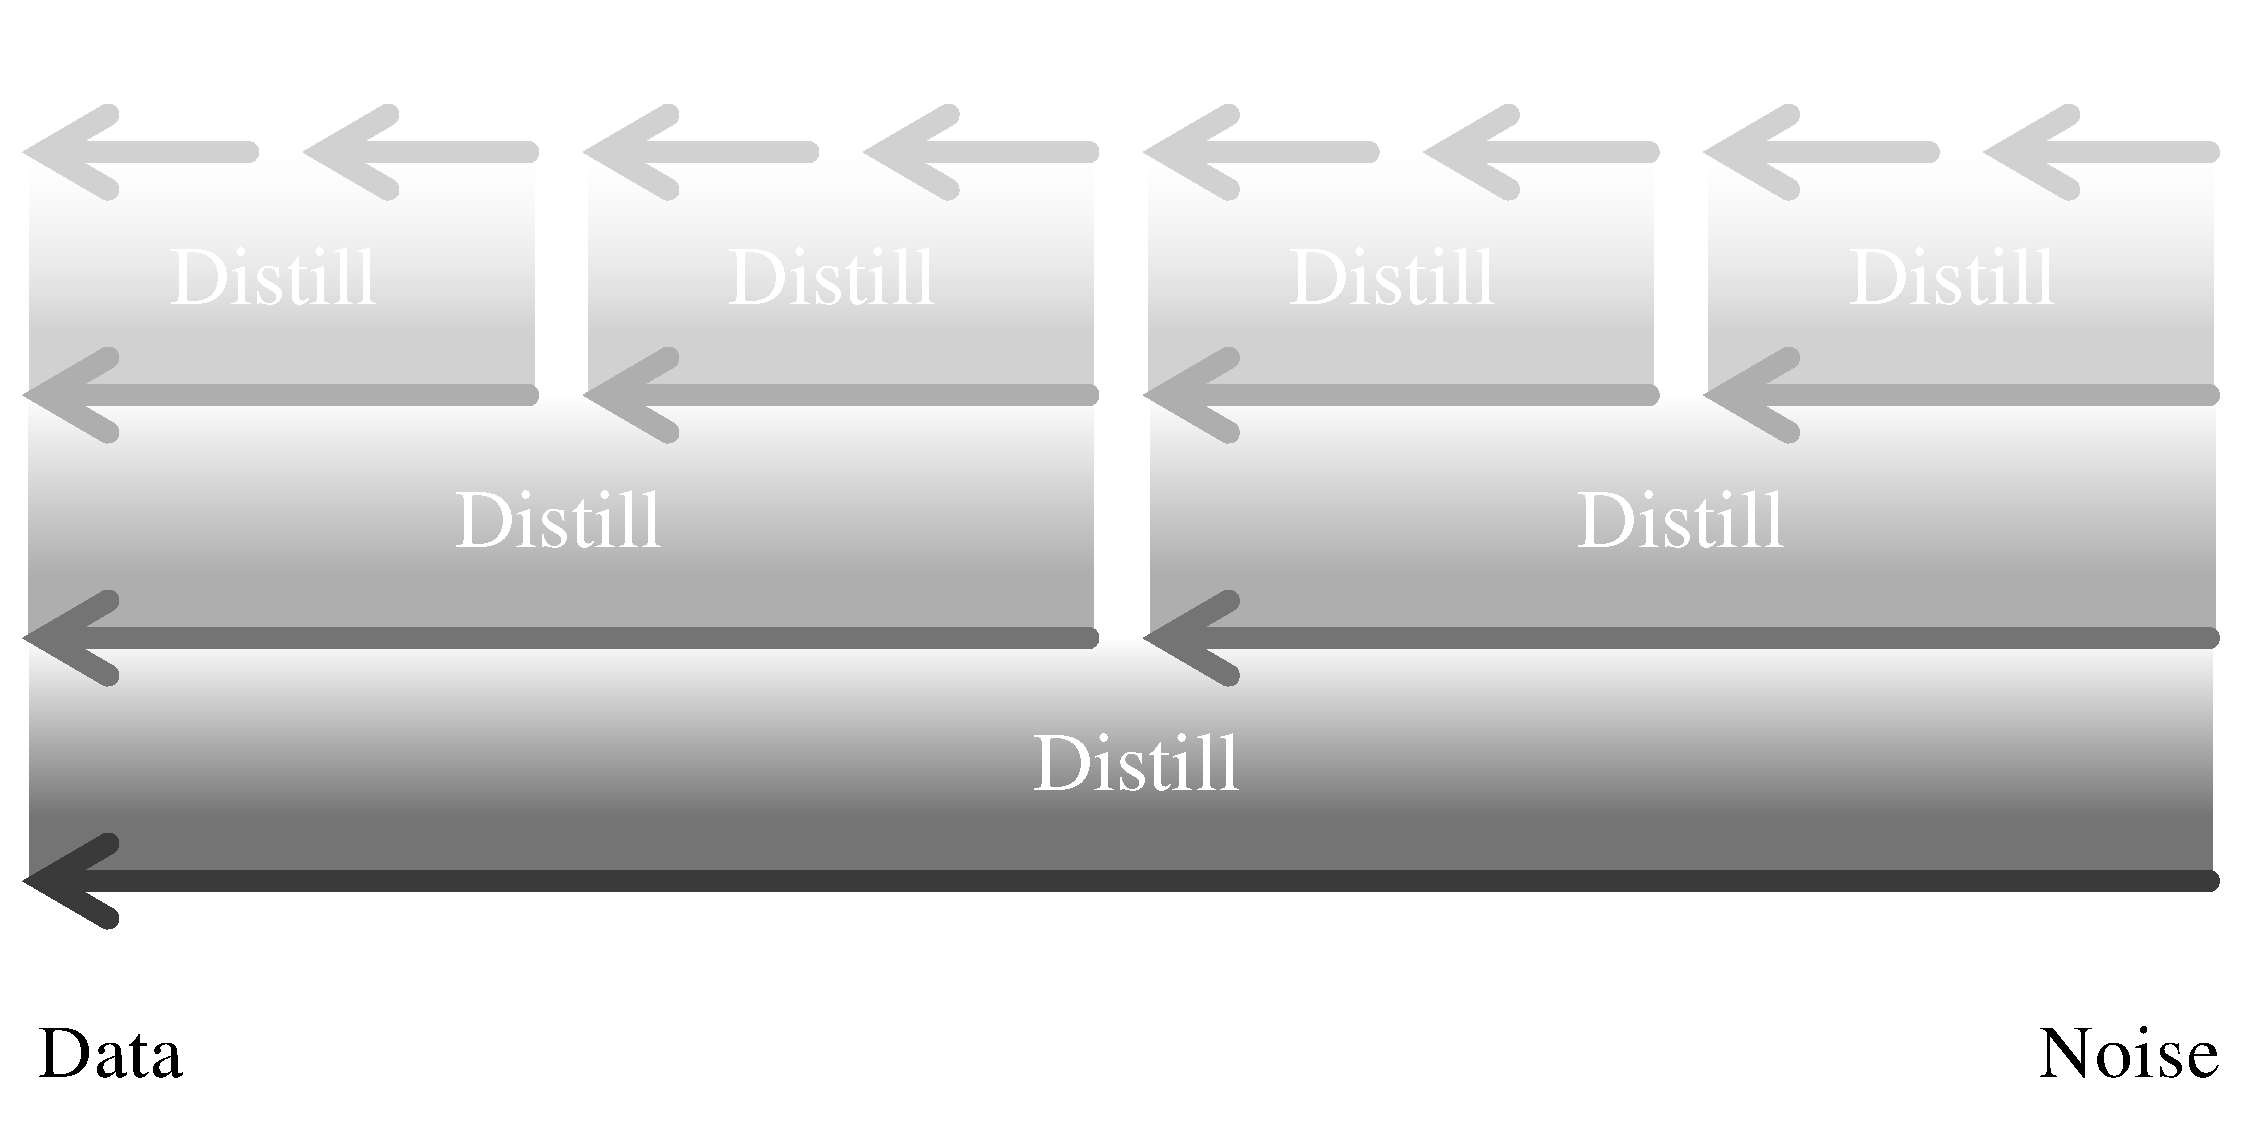
\includegraphics[width=0.93\linewidth]{Images/PartD/PD.pdf} 
    \caption{\textbfs{渐进式蒸馏（PD）示意图。}
在每一轮中，训练学生模型使得单步即可复现两个相邻教师步的效果。
该过程将 $N$ 个教师步蒸馏为 $N/2$ 个学生步，重复该过程可逐步将轨迹长度减半，直到达到所需的步数。
箭头表示多步教师转移如何被压缩为更少的学生步，从数据指向噪声。
\figcredit{由作者绘制。}
}
    \label{fig:pd-illustration}
\end{figure}



我们首先在 \Cref{subsec:pd-distillation} 中介绍 PD 的蒸馏操作，然后在 \Cref{subsec:pd-training} 中总结整个训练流程。\Cref{subsec:pd-guidance} 给出 CFG 引导的扩展。


\subsection{PD 中的蒸馏操作}\label{subsec:pd-distillation}

本节中，我们将 $\rvx$-预测参数化下的 DDIM 固定为时间步进规则，并仍将当前教师 $\rvx$-去噪器代入 DDIM 所得的确定性映射记为 $\mathtt{Solver}_{s \to t}$。


在第一轮 PD（教师 = 预训练扩散模型）中，这与通过 DDIM 积分扩散 PF-ODE 一致；在后续轮次（教师 = 上一轮学生）中，$\mathtt{Solver}_{s \to t}$ 仅仅是当前教师所诱导的 DDIM 转移，而非原始的扩散 PF-ODE。


蒸馏步骤如下：从带噪输入 $\rvx_s$（干净数据 $\rvx_s = \alpha_s \rvx_0 + \sigma_s \bm{\epsilon}$ 的扰动版本）出发，训练学生模型预测一个目标 ${\color{orange}\tilde\rvx}$，使得单步学生步 $s\!\to\! t$ 复现教师模型的两个连续步 $s\!\to\! u\!\to\! t$。
设 $\rvx_{\bm{\phi}^\times}(\rvx,\tau)$ 为本轮教师的 $\rvx$-预测去噪器。
将教师诱导的 DDIM 转移应用两次，得到
\[
\tilde\rvx_u := \mathtt{Solver}_{s\to u}\!\left(\rvx_s;\,\rvx_{\bm{\phi}^\times}\right),
\qquad
\tilde\rvx_t := \mathtt{Solver}_{u\to t}\!\left(\tilde\rvx_u;\,\rvx_{\bm{\phi}^\times}\right).
\]
这里我们使用 \Cref{eq:solver} 的记号，表示将 $\rvx_{\bm{\phi}^\times}$ 代入 DDIM 所诱导的、从 $s$ 到 $t$（以 $\rvx_s$ 为起点）的确定性转移映射。

\begin{question}
时间 $s$ 处的伪干净目标 ${\color{orange}\tilde\rvx}$ 是什么，使得求解器直接从 $s \to t$ 步进时产生与 $s \to u \to t$ 相同的输出 $\tilde\rvx_t$？具体而言，求满足下式的 ${\color{orange}\tilde\rvx}$：
\[
\tilde\rvx_t = \mathtt{Solver}_{s\to t}\left(\rvx_s; {\color{orange}\tilde\rvx}\right).
\]
\end{question}




一旦得到 ${\color{orange}\tilde\rvx}$ 的闭式表达，我们就训练一个学生模型 $\rvf_{\bm{\theta}}(\rvx_s, s)$（此处也是 $\rvx$-预测模型）来逼近“两步合一”目标 ${\color{orange}\tilde\rvx}$，最小化
\begin{align}\label{eq:pd-optimization}
\min_{\bm{\theta}} \E_s
\mathbb{E}_{\rvx_s\sim p_s}\!\left[w(\lambda_s)\,\big\|\rvf_{\bm{\theta}}(\rvx_s, s) - {\color{orange}\tilde\rvx}\big\|_2^2\right].
\end{align}


下面我们证明，DDIM 规则可通过初等代数给出 ${\color{orange}\tilde\rvx}$ 的闭式表达（注意该结果对离散时间和连续时间均成立）：
\lemp{DDIM 的“两步合一”目标 ${\color{orange}\tilde\rvx}$}{pd-ddim}{从初始条件 $\rvx_s$ 出发，若求解器取为 DDIM，则“两步合一”目标 ${\color{orange}\tilde\rvx}$ 可计算为
\begin{align*}
    {\color{orange}\tilde\rvx} 
    &=\frac{\sigma_s}{\alpha_t\sigma_s - \alpha_s\sigma_t} \tilde\rvx_t - \frac{\sigma_t}{\alpha_t\sigma_s - \alpha_s\sigma_t} \rvx_s.
\end{align*}
其中 $\tilde\rvx_t$ 由对 DDIM（\Cref{eq:ddim-update-all}）应用两次得到，路径为 $s \to u \to t$：
\begin{align*}
    s \to u: & \quad    && \tilde\rvx_u = \frac{\sigma_u}{\sigma_s}\rvx_s + \alpha_s \left(\frac{\alpha_u}{\alpha_s} - \frac{\sigma_u}{\sigma_s} \right)\rvx_{\bm{\phi}^\times}(\rvx_s, s)  \\
    u \to t: & \quad    && \tilde\rvx_t = \frac{\sigma_t}{\sigma_u}\tilde\rvx_u + \alpha_u \left(\frac{\alpha_t}{\alpha_u} - \frac{\sigma_t}{\sigma_u} \right)\rvx_{\bm{\phi}^\times}(\tilde\rvx_u, u).
\end{align*}
}{$\tilde\rvx_t$ 必须与从 $s$ 到 $t$ 的一步 DDIM $\tilde\rvx_t'$ 相匹配，其表达为：
\[
s \to t: \quad \tilde\rvx_t' = \frac{\sigma_t}{\sigma_s}\rvx_s + \alpha_s \left(\frac{\alpha_t}{\alpha_s} - \frac{\sigma_t}{\sigma_s} \right) {\color{orange}\tilde\rvx}.
\]
令 $\tilde\rvx_t'$ 与 $\tilde\rvx_t$ 相等，可解出 ${\color{orange}\tilde\rvx}$ 关于 $\tilde\rvx_t$、$s$、$t$ 的表达式：
\begin{align}
    &\tilde\rvx_t = \tilde\rvx_t' \nonumber \\
    \Longleftrightarrow\,\, & \tilde\rvx_t = \frac{\sigma_t}{\sigma_s}\rvx_s + \alpha_s \left(\frac{\alpha_t}{\alpha_s} - \frac{\sigma_t}{\sigma_s} \right) {\color{orange}\tilde\rvx} \nonumber \\
    \Longleftrightarrow\,\, & {\color{orange}\tilde\rvx} =  \frac{\tilde\rvx_t - \frac{\sigma_t}{\sigma_s}\rvx_s}{\alpha_s \left(\frac{\alpha_t}{\alpha_s} - \frac{\sigma_t}{\sigma_s} \right)} \label{eq:x-pd-paper} \\
    \Longleftrightarrow\,\, & {\color{orange}\tilde\rvx} = \frac{\sigma_s}{\alpha_t\sigma_s - \alpha_s\sigma_t} \tilde\rvx_t - \frac{\sigma_t}{\alpha_t\sigma_s - \alpha_s\sigma_t} \rvx_s. \nonumber
\end{align}
}
利用该公式，PD 在时间 $s$ 处计算伪干净目标，使其单步 DDIM 步进 $s\!\to\!t$ 恰好落到两步输出 $\tilde\rvx_t$。


\paragraph{实用的离散时间网格与损失。}
实践中，我们固定一个递减网格 $t_0=T>t_1>\cdots>t_N=0$，并为简洁记 $s:=t_k$，$u:=t_{k+1}$，$t:=t_{k+2}$。
教师模型提供单步映射 $\mathtt{Teacher}_{t_k\to t_{k+1}}$，学生模型学习一个两步跨越映射以匹配教师复合：
\[
\mathtt{Student}_{t_k\to t_{k+2}}
 \approx 
\mathtt{Teacher}_{t_{k+1}\to t_{k+2}}
\circ
\mathtt{Teacher}_{t_{k}\to t_{k+1}}.
\]

我们采样三元组 $(s,u,t)=(t_k,t_{k+1},t_{k+2})$，其中 $k\in\{0,\ldots,N-2\}$。
目标 \Cref{eq:pd-optimization} 变为
\[
\min_{\bm{\theta}} 
\mathbb{E}_{\,k \sim \mathcal{U}[\![0,N{-}2]\!]}\,
\mathbb{E}_{\,\rvx_{t_k}\sim p_{t_k}}\!
\Big[
  w(\lambda_{t_k})\,
  \big\|
  \rvf_{\bm{\theta}}(\rvx_{t_k},t_k) - {\color{orange}\tilde\rvx}^{(k)}
  \big\|_2^2
\Big],
\]
其中教师两步目标 ${\color{orange}\tilde\rvx}^{(k)}$ 通过引理~\ref{pd-ddim} 计算。若网格均匀，可写 $t_k = T(1 - k/N)$，从而
\[
s = T\Big(1 - \frac{k}{N}\Big),\quad
u = T\Big(1 - \frac{k+1}{N}\Big),\quad
t = T\Big(1 - \frac{k+2}{N}\Big),
\]
对应于步长 $\Delta s =  T/N$ 的均匀间隔时间步。


\subsection{PD 的完整训练流程及其采样}\label{subsec:pd-training}
通过 \Cref{eq:pd-optimization} 在局部配对片段上训练后，$\mathtt{Student}$ 不再沿原始网格的每个区间前进。相反，每个学习到的步覆盖两个连续的 $\mathtt{Teacher}$ 步，因此 $\mathtt{Student}$ 在每隔一个时间点上前进，
\[
t_0 \to t_2 \to t_4 \to \cdots \to t_N,
\]
从而仅用 $N/2$ 次转移即可遍历相同的跨度 $[0,T]$。此阶段之后，训练好的 $\mathtt{Student}$ 取代 $\mathtt{Teacher}$ 作为新的去噪器模型。然后该流程在更稀疏的网格（时间步长加倍）上重复，得到递进
\[
N \;\to\; N/2 \;\to\; N/4 \;\to\; \cdots,
\]
直到达到所需的推理步数。每次迭代中，新的 $\mathtt{Student}$ 由更新后的 $\mathtt{Teacher}$ 初始化。这种迭代式减半在保持全局时间跨度的同时，逐步压缩生成过程的时间分辨率。

\paragraph{采样。}
在推理时，使用当前 $\mathtt{Student}$ 作为去噪器的（DDIM）求解器，采样器在训练所诱导的稀疏网格上前进。第一轮后它做“跳 2”跳跃（$t_0 \to t_2 \to \cdots \to t_N$），下一轮后做“跳 4”（$t_0 \to t_4 \to \cdots \to t_N$），以此类推，每次迭代都将采样步数减半，同时保持相同的起止时间。

\subsection{补充讨论：局部半群匹配与广义求解器的可能性}


\paragraph{作为局部半群匹配的渐进式蒸馏。}
在统一目标 \Cref{eq:general-cm-loss} 中，不可处理的 oracle
目标 $\bPsi_{s\to 0}$ 被一个教师诱导的代理所替代，该代理使用
ODE 流的\emph{半群性质}（详见后文 \Cref{eq:semi-group}）：从 $s$ 演化到 $t$ 应当
等价于先从 $s$ 到任意中间点 $u$，再从 $u$ 到 $t$，
\[
\bPsi_{s\to t} = \bPsi_{u\to t}\circ\bPsi_{s\to u}.
\]
PD 通过训练学生单步映射匹配教师两个相邻单步片段的复合来局部地施加这一点：
\begin{align}\label{eq:pd-local}
  \E_{s}\E_{\rvx_s\sim p_s}
  \big\|
    \underbrace{\rmG_{\btheta}(\rvx_s, s, s-2\Delta s)}_{\text{student one-step}}
    -
    \underbrace{\mathtt{Solver}_{s-\Delta s\to s-2\Delta s}\big(\mathtt{Solver}_{s\to s-\Delta s}(\rvx_s)\big)}_{\text{teacher two-step composition}}
  \big\|_2^2.
\end{align}
最小化 \Cref{eq:pd-local} 在一个短递减网格上实例化半群恒等式（取 $s>u>t$，$u=s-\Delta s$，$t=s-2\Delta s$）：
\begin{align*}
  \bPsi_{s\to s-2\Delta s}
  &= \bPsi_{s-\Delta s\to s-2\Delta s}\circ\bPsi_{s\to s-\Delta s}
  \\&\approx
  \mathtt{Solver}_{s-\Delta s\to s-2\Delta s}\circ \mathtt{Solver}_{s\to s-\Delta s},
\end{align*}
因此训练只需要短的教师片段，而无需从时间 $s$ 一直
展开到 $0$。

为与 \Cref{eq:general-cm-loss} 中的少步去噪器视角联系起来，将
学生模型的少步映射定义为已学跳跃的复合：
\[
\underbrace{\rmG_{\btheta}(\rvx_s, s, 0)}_{\text{few-step denoiser}}
=
\big(\rmG_{\btheta}(\,\cdot\,, 2\Delta s, 0)\circ\cdots\circ \rmG_{\btheta}(\,\cdot\,, s, s-2\Delta s)\big)(\rvx_s).
\]
从概念上讲，\Cref{eq:pd-local} 为全局回归
\[
\E_{s,\rvx_s}\Big\|\rmG_{\btheta}(\rvx_s,s,0)\;-\;(\mathtt{Solver})^{\circ}_{s\to 0}(\rvx_s)\Big\|_2^2,
\]
提供了一个高效的\emph{局部代理}，
其中 $(\mathtt{Solver})^{\circ}_{s\to 0}$ 表示教师在步长为 $\Delta s$ 的网格上从 $s$ 到 $0$ 的完整
复合，作为 $\bPsi_{s\to 0}$ 的代理。

\paragraph{能否使用其他求解器？}
在上面对 PD 的介绍中，我们以 $\rvx$-预测参数化下的 DDIM 为具体的 PF-ODE 采样器进行了重点讨论。
带网格减半的局部半群匹配在确定性状态到状态映射的层面上是求解器无关的，并在参数化（$\rvx$、$\beps$、$\rvv$、score）之间进行标准转换后，可扩展到 \Cref{ch:solvers} 中的时间步进方法。
然而，此处的闭式伪目标依赖于\emph{单步、显式}更新，其单步映射对回归目标是\emph{仿射}的（如 DDIM 以及应用于 PF-ODE 的指数 Euler 或显式 RK 等显式单步格式）。
对于\emph{多步}或\emph{隐式}求解器（需要步历史或内层求解），应改为直接匹配相应的转移映射（参见 \Cref{eq:pd-local}）并提供必要的历史或热启动；一般而言不存在可比的闭式反演。

若采样器是随机的，则对每个样本固定噪声序列以获得确定性转移
$\mathtt{Teacher}^{(\omega)}_{s\to t}$（其中 $\omega$ 为固定的噪声种子）。
在这种情况下，PD 回归于一个固定的转移映射；闭式伪目标通常要求单步显式仿射更新；否则使用 \Cref{eq:pd-local} 中的直接匹配。









% In this section, we focus on DDIM in the $\rvx$-prediction parameterization as a concrete time–stepping rule.
% Here, $\mathtt{Solver}_{s \to t}$ denotes the current teacher’s deterministic transition map from $s$ to $t$, obtained by plugging the teacher denoiser into the same fixed update rule (DDIM).

% In the first PD round (teacher = pre–trained diffusion model), this coincides with integrating the diffusion PF–ODE via DDIM.
% In later rounds (teacher = previous student), $\mathtt{Solver}_{s \to t}$ remains the DDIM update induced by the current teacher denoiser; we do not identify it with the original diffusion PF–ODE.

% The distillation step is as follows: starting from a noisy input $\rvx_s$ (a perturbed version of clean data, $\rvx_s = \alpha_s \rvx_0 + \sigma_s \bm{\epsilon}$), the student is trained to predict a target ${\color{orange}\tilde\rvx}$ such that a single student step matches two teacher steps. More precisely, consider timesteps $s \to u \to t$, starting from $\rvx_s$.
% Let $\rvx_{\bm{\phi}^\times}(\rvx,\tau)$ denote the teacher’s $\rvx$-prediction denoiser in this round.
% Applying the teacher–induced DDIM transition twice gives
% \[
% \tilde\rvx_u := \mathtt{Solver}_{s\to u}\!\left(\rvx_s;\,\rvx_{\bm{\phi}^\times}\right),
% \qquad
% \tilde\rvx_t := \mathtt{Solver}_{u\to t}\!\left(\tilde\rvx_u;\,\rvx_{\bm{\phi}^\times}\right).
% \]
% Here, we use the notation of \Cref{eq:solver} to denote the deterministic transition map from $s$ to $t$ (starting at $\rvx_s$) induced by plugging $\rvx_{\bm{\phi}^\times}$ into DDIM.

% \begin{question}
% What is the pseudo-clean ${\color{orange}\tilde\rvx}$ at time $s$ such that the solver produces the same output $\tilde\rvx_t$ when stepping directly $s \to t$ as it does via $s \to u \to t$? Specifically, determine ${\color{orange}\tilde\rvx}$ satisfying:
% \[
% \tilde\rvx_t = \mathtt{Solver}_{s\to t}\left(\rvx_s; {\color{orange}\tilde\rvx}\right).
% \]
% \end{question}

% Once a closed-form expression for ${\color{orange}\tilde\rvx}$ is obtained, we train a student model $\rvf_{\bm{\theta}}(\rvx_s, s)$ (also an $\rvx$-prediction model here) to approximate the ``two-steps-in-one'' target ${\color{orange}\tilde\rvx}$ by minimizing
% \begin{align}\label{eq:pd-optimization}
% \min_{\bm{\theta}}\;
% \mathbb{E}_{\rvx_s\sim p_s}\!\left[w(\lambda_s)\,\big\|\rvf_{\bm{\theta}}(\rvx_s, s) - {\color{orange}\tilde\rvx}\big\|_2^2\right].
% \end{align}

% In the following, we show that the DDIM rule yields ${\color{orange}\tilde\rvx}$ in closed form via elementary algebra:
% \lemp{Two-Steps-in-One Target ${\color{orange}\tilde\rvx}$ of DDIM}{pd-ddim}{Starting from an initial condition $\rvx_s$, if the solver is taken as DDIM, then the ``two-step-in-one'' target ${\color{orange}\tilde\rvx}$ can be computed as
% \begin{align*}
%     {\color{orange}\tilde\rvx} 
%     % &=      \frac{\tilde\rvx_t - \frac{\sigma_t}{\sigma_s}\rvx_s  }{\alpha_s \left(\frac{\alpha_t}{\alpha_s} - \frac{\sigma_t}{\sigma_s} \right)} \\
%     &=\frac{\sigma_s}{\alpha_t\sigma_s - \alpha_s\sigma_t} \tilde\rvx_t - \frac{\sigma_t}{\alpha_t\sigma_s - \alpha_s\sigma_t} \rvx_s.
% \end{align*}
% Here, $\tilde\rvx_t$ is obtained by applying DDIM (in \Cref{eq:ddim-update-all}) twice, from $s \to u \to t$:
% \begin{align*}
%     s \to u: & \quad    && \tilde\rvx_u = \frac{\sigma_u}{\sigma_s}\rvx_s + \alpha_s \left(\frac{\alpha_u}{\alpha_s} - \frac{\sigma_u}{\sigma_s} \right)\rvx_{\bm{\phi}^\times}(\rvx_s, s)  \\
%     u \to t: & \quad    && \tilde\rvx_t = \frac{\sigma_t}{\sigma_u}\tilde\rvx_u + \alpha_u \left(\frac{\alpha_t}{\alpha_u} - \frac{\sigma_t}{\sigma_u} \right)\rvx_{\bm{\phi}^\times}(\tilde\rvx_u, u).
% \end{align*}
% }{$\tilde\rvx_t$ must be matched with the one-step DDIM from $s$ to $t$, $\tilde\rvx_t'$, expressed as:
% \[
% s \to t: \quad \tilde\rvx_t' = \frac{\sigma_t}{\sigma_s}\rvx_s + \alpha_s \left(\frac{\alpha_t}{\alpha_s} - \frac{\sigma_t}{\sigma_s} \right) {\color{orange}\tilde\rvx}.
% \]
% By equating $\tilde\rvx_t'$ and $\tilde\rvx_t$, we can solve for ${\color{orange}\tilde\rvx}$ in terms of $\tilde\rvx_t$, $s$, and $t$:
% \begin{align}
%     &\tilde\rvx_t = \tilde\rvx_t' \nonumber \\
%     \Longleftrightarrow\,\, & \tilde\rvx_t = \frac{\sigma_t}{\sigma_s}\rvx_s + \alpha_s \left(\frac{\alpha_t}{\alpha_s} - \frac{\sigma_t}{\sigma_s} \right) {\color{orange}\tilde\rvx} \nonumber \\
%     \Longleftrightarrow\,\, & {\color{orange}\tilde\rvx} =  \frac{\tilde\rvx_t - \frac{\sigma_t}{\sigma_s}\rvx_s}{\alpha_s \left(\frac{\alpha_t}{\alpha_s} - \frac{\sigma_t}{\sigma_s} \right)} \label{eq:x-pd-paper} \\
%     \Longleftrightarrow\,\, & {\color{orange}\tilde\rvx} = \frac{\sigma_s}{\alpha_t\sigma_s - \alpha_s\sigma_t} \tilde\rvx_t - \frac{\sigma_t}{\alpha_t\sigma_s - \alpha_s\sigma_t} \rvx_s. \nonumber
% \end{align}
% }
% With this formula, PD inverts a single DDIM update to compute the target value that the student must predict so that one student step arrives at ${\color{orange}\tilde\rvx}$.

% In practice, the discrete timestep $i$ is drawn uniformly as $i \sim \mathcal{U}[\![1,N]\!]$, and rescaled as
% \[
% s = \tfrac{i}{N}, \quad u = s - \tfrac{1}{2N}, \quad t = s - \tfrac{1}{N}.
% \]
% Thus, after the first distillation iteration, the teacher’s $N$-step sampler is compressed into a student model with $N/2$ steps.



% \subsection{Entire Training Pipeline of PD}\label{subsec:pd-training}
% After distilling the $2N$ steps of the teacher model into $N$ steps in the student model $\rmG_{\bm{\theta}}$ using \Cref{eq:pd-optimization}, the resulting $N$-step student model can be utilized as the new teacher. The same distillation procedure is then repeated to further distill the new teacher model into an $N/2$-step student model. At each iteration, the new student model is initialized with the parameters of the updated teacher model. This distillation process is progressively applied over multiple iterations.

% \paragraph{Sampling.}
% With the new student model serving as a denoiser in the empirical PF-ODE, the number of required sampling steps is halved at each iteration by utilizing the (DDIM) solver.


% \paragraph{Progressive Distillation as Local Semigroup Matching.}
% Within the unified objective \Cref{eq:general-cm-loss}, the intractable oracle
% target $\bPsi_{s\to 0}$ is replaced by a teacher–induced surrogate that uses the
% \emph{semigroup property} of the ODE flow (see more details later in \Cref{eq:semi-group}): evolving from $s$ to $t$ should be
% equivalent to going from $s$ to any intermediate $u$ and then from $u$ to $t$,
% \[
% \bPsi_{s\to t} \;=\; \bPsi_{u\to t}\circ\bPsi_{s\to u}.
% \]
% PD enforces this locally by training the student’s one–step map to match the
% teacher’s composition of two adjacent one–step fragments:
% \begin{align}\label{eq:pd-local}
%   \E_{s}\E_{\rvx_s\sim p_s}
%   \big\|
%     \underbrace{\rmG_{\btheta}(\rvx_s, s, s-2\Delta s)}_{\text{student one step}}
%     -
%     \underbrace{\mathtt{Solver}_{s-\Delta s\to s-2\Delta s}\big(\mathtt{Solver}_{s\to s-\Delta s}(\rvx_s)\big)}_{\text{teacher two-step composition}}
%   \big\|_2^2.
% \end{align}
% Minimizing \Cref{eq:pd-local} instantiates the semigroup identity on a short
% decreasing grid (take $s>u>t$ with $u=s-\Delta s$ and $t=s-2\Delta s$):
% \begin{align*}
%   \bPsi_{s\to s-2\Delta s}
%   &= \bPsi_{s-\Delta s\to s-2\Delta s}\circ\bPsi_{s\to s-\Delta s}
%   \\&\approx
%   \mathtt{Solver}_{s-\Delta s\to s-2\Delta s}\circ \mathtt{Solver}_{s\to s-\Delta s},
% \end{align*}
% so training only requires short teacher fragments, rather than a full rollout
% from time $s$ all the way to $0$.

% To connect back to the few–step denoiser view in \Cref{eq:general-cm-loss}, define
% the student’s few–step map as a composition of learned jumps:
% \[
% \underbrace{\rmG_{\btheta}(\rvx_s, s, 0)}_{\text{few-step denoiser}}
% =
% \big(\rmG_{\btheta}(\,\cdot\,, 2\Delta s, 0)\circ\cdots\circ \rmG_{\btheta}(\,\cdot\,, s, s-2\Delta s)\big)(\rvx_s).
% \]
% Conceptually, \Cref{eq:pd-local} provides an efficient \emph{local surrogate} for the
% global regression
% \[
% \E_{s,\rvx_s}\Big\|\rmG_{\btheta}(\rvx_s,s,0)\;-\;(\mathtt{Solver})^{\circ}_{s\to 0}(\rvx_s)\Big\|_2^2,
% \]
% where $(\mathtt{Solver})^{\circ}_{s\to 0}$ denotes the teacher’s full
% composition from $s$ to $0$ on a grid with step size $\Delta s$, serving as a
% proxy for $\bPsi_{s\to 0}$.

% In practice, PD proceeds by grid halving: start from an $N$–step teacher
% ($\Delta s=T/N$), learn $\rmG_{\btheta}(\,\cdot\,,\cdot,\,\cdot-2\Delta s)$ via
% \Cref{eq:pd-local} to obtain an $N$–step student, set this student as the new
% teacher, and iterate $N\to N/2\to N/4\to \cdots$ until reaching the
% target step count.



\subsection{带引导的 PD}\label{subsec:pd-guidance}
\citet{meng2023distillation} 提出了一种两阶段流程，用于蒸馏
无分类器引导（CFG）扩散模型：(1) 将引导\emph{蒸馏}
到一个以引导权重为输入的单网络中，(2) 应用
\emph{渐进式蒸馏（PD）}以减少采样步数。他们在像素空间和隐空间（如 Stable Diffusion）中均
验证了该方法。

\paragraph{第一阶段蒸馏：蒸馏引导。}
设 $\rvx_{\bm{\phi}^\times}(\rvx_s, s, \rvc)$ 为（预训练）条件
扩散模型在“$\rvx$-预测”参数化下（即干净估计）于时间 $s$、条件 $\rvc$ 处的输出；条件也可以
为空，$\rvc=\emptyset$（无条件分支）。\Cref{eq:cfg-model-nn} 中 $\omega$ 加权的 CFG
组合可写为
\begin{equation}\label{eq:cfg-model-clean}
   \rvx_{\bm{\phi}^\times}^{\,\omega}(\rvx_s, s, \rvc)
   := (1+\omega)\,\rvx_{\bm{\phi}^\times}(\rvx_s, s, \rvc)
      - \omega\,\rvx_{\bm{\phi}^\times}(\rvx_s, s, \emptyset),
\end{equation}
其中 $\omega \sim p_\omega(\omega)$，$p_\omega$ 为某个 CFG 加权分布，通常 $p_\omega(\omega)=\mathcal{U}[\omega_{\min},\omega_{\max}]$。

第一阶段引入一个新模型 $\rvx_{\bm{\theta}_1}(\rvx_s, s, \rvc, \omega)$，
它直接以 $\omega$ 为输入，通过监督
回归学习复现 CFG 输出 $\rvx_{\bm{\phi}^\times}^{\,\omega}(\rvx_s, s, \rvc)$：
\[
\min_{\bm{\theta}_1}\;
\mathbb{E}_{\omega\sim p_\omega, s, \rvx\sim p_{\mathrm{data}}, \rvx_s \sim p(\rvx_s\mid \rvx)}
\lambda(s)
\big\|\rvx_{\bm{\theta}_1}(\rvx_s, s, \rvc, \omega)-\rvx_{\bm{\phi}^\times}^{\omega}(\rvx_s, s, \rvc)\big\|_2^2.
\]
此处 $\lambda(s)$ 是标准的依赖调度的加权；每次迭代采样 $\omega$
教会单个网络在任意引导强度下模拟 CFG。

\paragraph{第二阶段蒸馏：PD。}
第一阶段模型 $\rvx_{\bm{\theta}_1}(\rvx_s, s, \rvc, \omega)$ 作为
PD 中的教师，按照 \Cref{subsec:pd-training} 被逐步蒸馏成一个采样步数更少的学生
$\rvx_{\bm{\theta}_2}(\rvx_s, s, \rvc, \omega)$。每次迭代步数
减半（例如 $N \to N/2 \to N/4 \to \cdots$）。

\newpage
\section{结语}\label{sec:ch10_cr}

本章介绍了我们的第一种主要的基于训练的加速范式。在通过数值求解器穷尽了无训练改进之后，我们将焦点转向一种新策略：训练一个快速的\textit{学生}生成器，使其学会复现一个缓慢、预训练的\textit{教师}扩散模型的行为。

我们探讨了两类主要的蒸馏思想。首先，在以 Variational Score Distillation（VSD）等为代表的分布级蒸馏中，通过在不同噪声水平上对齐各自的分数函数，训练学生模型的输出分布去匹配教师模型的分布，从而提供一个稳定、非对抗的目标。其次，在流映射蒸馏中，我们看到像渐进式蒸馏（PD）这样的方法训练学生模型直接逼近教师模型的解轨迹。PD 的迭代式方法——每一轮将采样步数减半——被证明是将一个漫长的迭代过程压缩为少数几步的强大而实用的方法。

这些蒸馏技术成功地弥合了迭代扩散模型的高样本质量与单步生成器推理速度之间的鸿沟，为高效、高保真合成提供了一条引人注目的路径。

然而，依赖预训练教师模型引入了两阶段流程：先训练一个缓慢但强大的教师，再将其蒸馏成一个快速的学生。这引出了生成式建模研究前沿的一个根本问题：我们能否完全绕过教师模型？

是否可能设计一种独立的训练原则，直接从数据学习这些快速的少步生成器？本书的最后一章将回答这个问题。
\begin{enumerate}
    \item 我们将探索诸如一致性模型（Consistency Models）等开创性方法，它们学习从 ODE 轨迹上任意一点到其终点之间的映射。
    \item 我们将深入探讨一致性模型的广义概念，它们学习在单步内将 ODE 轨迹上任意一点映射到另一点。
\end{enumerate}

这种从改进求解器或蒸馏解到直接学习解映射本身的转变，代表了向一类既原理化又在设计上高度高效的新型生成模型迈出的重要一步。

\clearpage
\newpage
